\documentclass[11pt]{article}
\usepackage{fullpage,amsmath,mathtools, algorithm2e, forest}
\usepackage[mathletters]{ucs}
\usepackage{hyperref}
\usepackage[utf8x]{inputenc}
\usepackage{graphicx}
\usepackage{listings}
\usepackage{courier}

\lstset{basicstyle=\footnotesize\ttfamily,breaklines=true}
\lstset{frame=single}

\graphicspath{ {./images/} }
\title{COMP4107 - Assignment 3}
\author{Student Name: Yunkai Wang\\
\text{Student Number: 100968473}\\\\
Student Name: Jules Kuehn\\
\text{Student Number: 100661464}}
\date{Fall 2018}
\begin{document}
\maketitle
\begin{enumerate}

\item
a) See q1.py for code. To see a comparison of input and output to the network, uncomment printVector() statements.\newline
\newline
In general, the fewer training images were used, the better the Hopfield network performed. These results suggests that a Hopfield network is a very poor choice for classification.\newline
A major factor in the accuracy was the selection of training images. Since fewer training images performed better, a random selection of a representative 1 or 5 leaves much to chance. To address this, we selected the training images with k-means, taking the images closest to the 2 cluster centers. This results in a selection of training images in which all 1's are very close to the center 1, and all 5's are very close to the center 5. This worked better than random selection, and didn't show the same sharp decline in classification accuracy as more training images were added.\newline
Alternately, we tried taking as many cluster centers as training images, finding the closest image for each cluster center. This should result in selecting training images that maximally differ from each other. This worked quite poorly as the quite different images caused further degeneration.\newline
The graphs below compare classification accuracy against the number of images used to train the network (between 1 and 5 of each digit). Each graph shows the average classification accuracy over 5 trials, with 50 test images.
% \begin{figure}[h!]
%     \centering
%      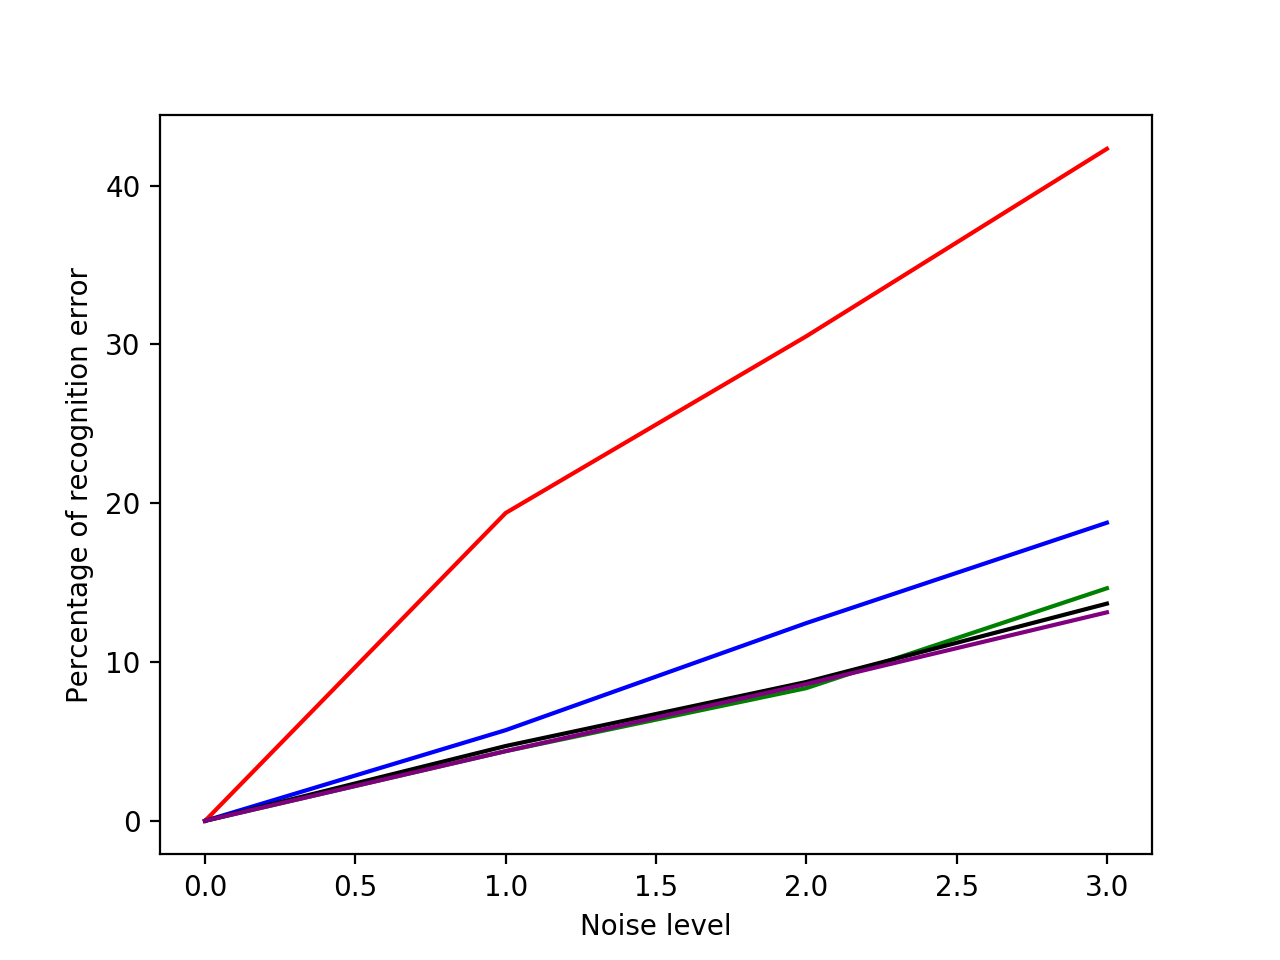
\includegraphics[width=0.5\textwidth]{q2-a-1}
%         \caption{Classification accuracy vs. number of training images}
% \end{figure}
% \lstinputlisting{python_output/q1a-results.txt}

b) The code to implement the Storkey improvements are also included in our q1.py code.\newline
\newline
As shown below, the Storkey algorithm does not substantially improve the results for the classification, even for the best case shown above (where)
% \begin{figure}[h!]
%     \centering
%      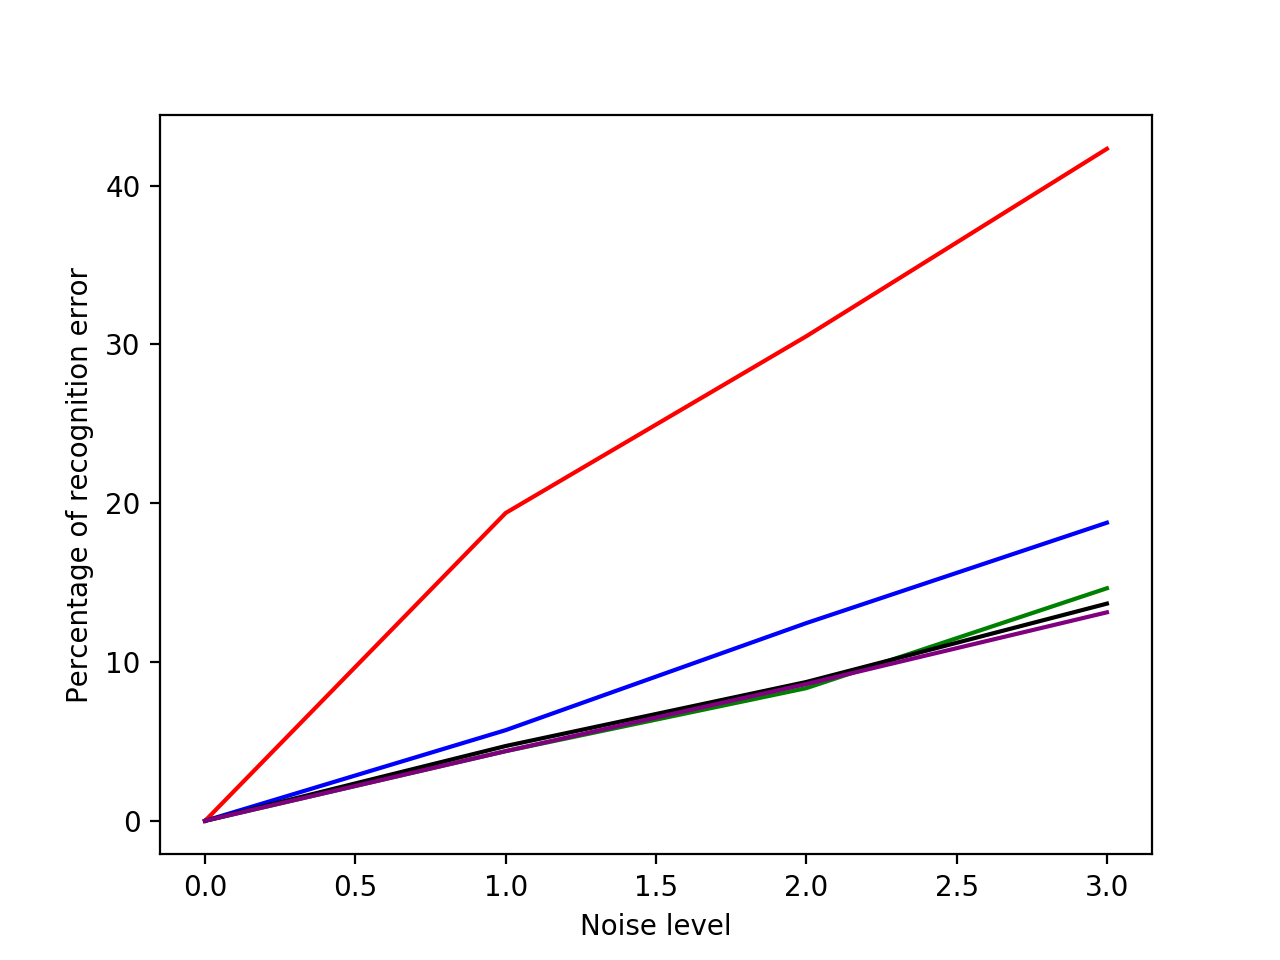
\includegraphics[width=0.5\textwidth]{q2-a-1}
%         \caption{With and without Storkey's rule}
% \end{figure}
% \lstinputlisting{python_output/q1b-results.txt}


c) We can further show that 8 neurons is a good choice by noting that early stopping has no effect. Our experiments have not been able to demonstrate an overtraining phenomenon with even 50 hidden neurons, but a premature early stop can be seen in Figure 6, and the table below.\newline
\lstinputlisting{python_output/q1c-results.txt}

\begin{figure}[h!]
    \centering
    \begin{minipage}{0.45\textwidth}
        \centering
        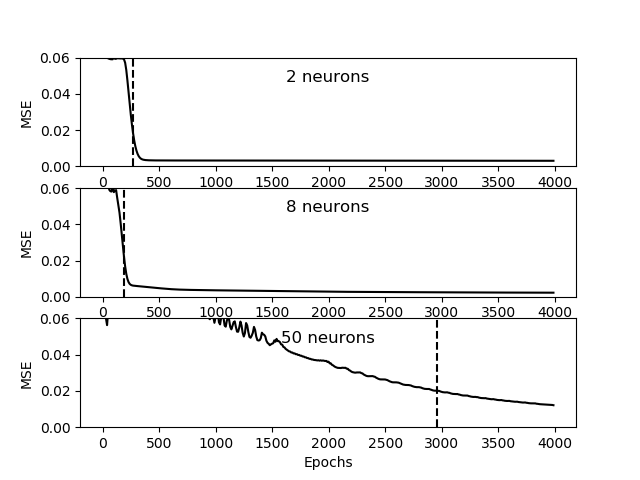
\includegraphics[width=0.9\textwidth]{q1c-1-50_neurons_slow_convergence2} % first figure itself
        \caption{Slow convergence}
    \end{minipage}\hfill
    \begin{minipage}{0.45\textwidth}
        \centering
        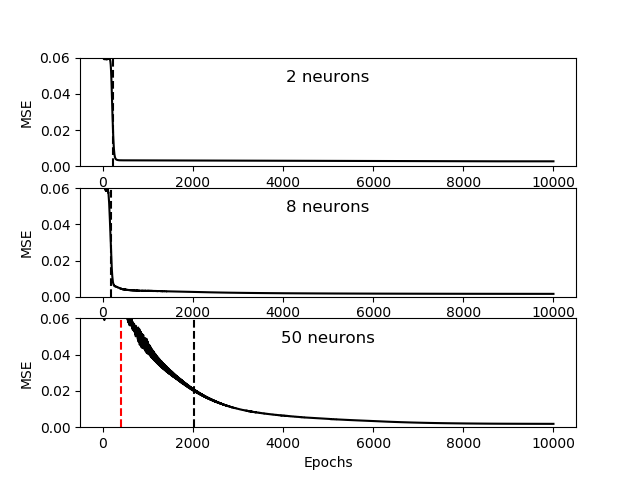
\includegraphics[width=0.9\textwidth]{q1c-2-earlyStopping} % second figure itself
        \caption{Premature early stop}
    \end{minipage}
\end{figure}

The network with 50 hidden neurons also is very slow to converge to the target MSE - even using the RMSPropOptimizer - compared to when using 8 hidden neurons (Figure 5).\newline

\begin{figure}[h!]
    \centering
    \begin{minipage}{0.45\textwidth}
        \centering
        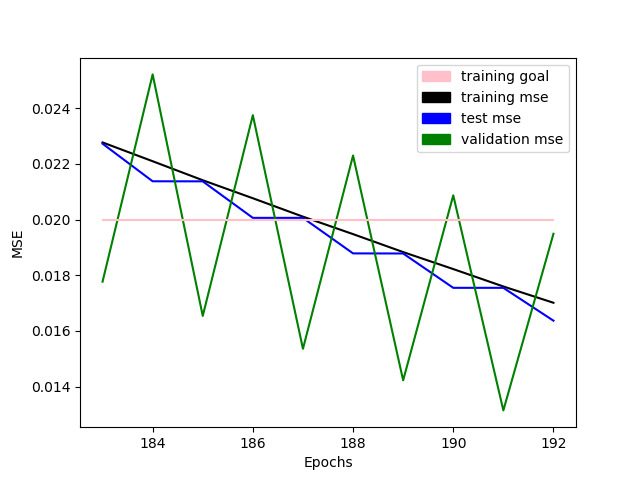
\includegraphics[width=0.9\textwidth]{q1c-3} % first figure itself
        \caption{Reaching training goal}
    \end{minipage}\hfill
    \begin{minipage}{0.45\textwidth}
        \centering
        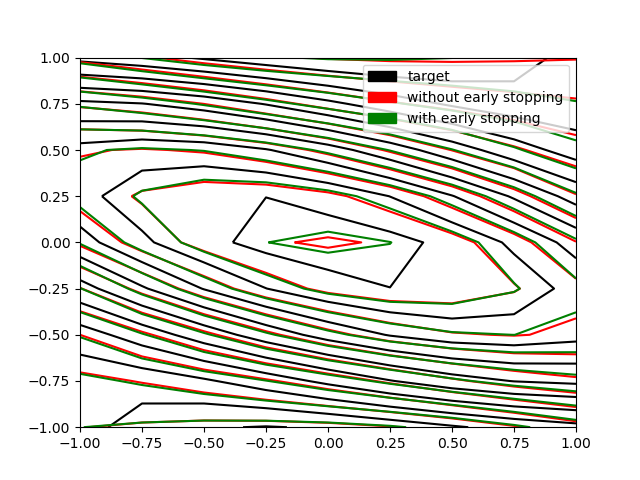
\includegraphics[width=0.9\textwidth]{q1c-32} % second figure itself
        \caption{Early stopping not triggered}
    \end{minipage}
\end{figure}

Figure 7 shows the MSE at each epoch near where the training goal is reached. This captures the expected trend - that the training error will decrease consistently, while the test error (9x9 grid) has more variation. The validation data is most different from the training data (as it is randomly sampled from the function), so it is expected that its error would also have the highest variance.\newline
\newline
Figure 8 shows that having an early stopping mechanism for this function makes no difference, as the early stopping mechanism is never triggered (8 hidden neurons, 4000 epochs, 0.02 LR). Thus, the two contours are virtually identical, differing only by the stochastic elements of the experiments (initial weights, order of training data). 

\pagebreak
\item Instructions on how to run q2.py:\newline
\newline
Running q2.py without changing anything will run all three parts. This may take a while as it runs 10 experiments for each number of hidden neurons, and after one is finished, a new neural net is created to run the second one, etc. Therefore, it will take about 1 min for it to finish and plot the graphs. To run a single part only, comment out the other lines in the experiment() function.\\
We started by using the default learning rate for AdamOptimizer (0.001). This took 400-700 epochs to converge to the result. However, if we use 0.01 as the learning rate, it converges faster -- within 100 epochs every time. Therefore, we chose 0.01 as the learning rate for this question.\\

% \lstinputlisting{python_output/q2.out}
% 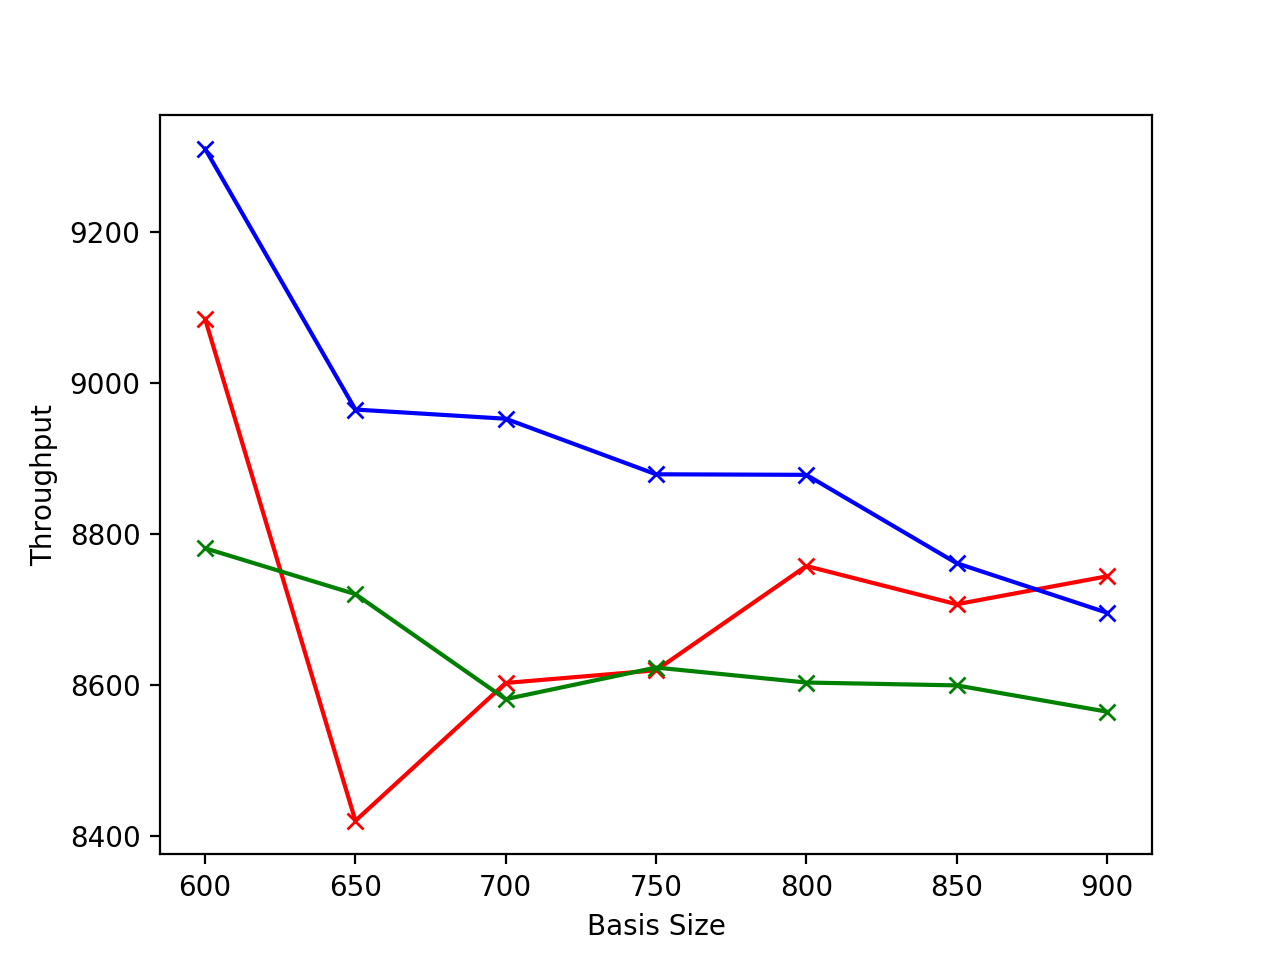
\includegraphics[width=0.7\columnwidth]{q7_result3}
\begin{enumerate}
\item We took the averages of 10 experiments for each of 5, 10, 15, 20, and 25 hidden neurons. The results are shown below.\newline

\begin{figure}[h!]
    \centering
     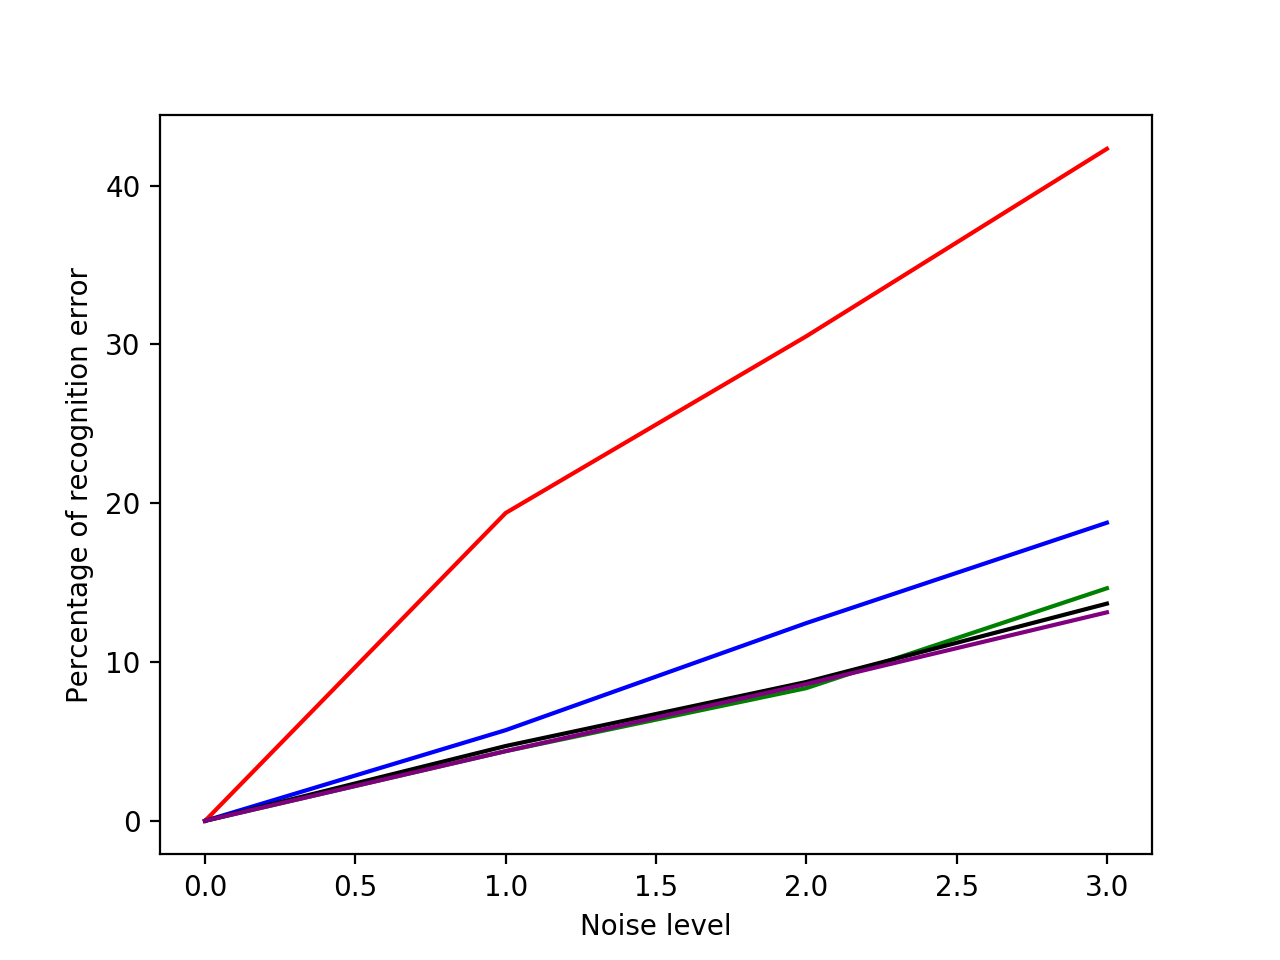
\includegraphics[width=0.5\textwidth]{q2-a-1}
        \caption{Percentage of Recognition Errors}
\end{figure}

The table below corresponds to the experiment shown in the graph above.\newline
\lstinputlisting{python_output/q2a-results.txt}

\item 15 is chosen as the number of hidden neurons, since 15 is more accurate than 10, but using more than 15 neurons is not much better (if at all). When we used 15 neurons in the hidden layer, the number of epochs to reach zero errors is much less than is shown in the assignment question, which we think is fine. Perhaps this is due to a different learning rate.\\
\begin{figure}[h!]
    \centering
    \begin{minipage}{0.45\textwidth}
    	\centering
        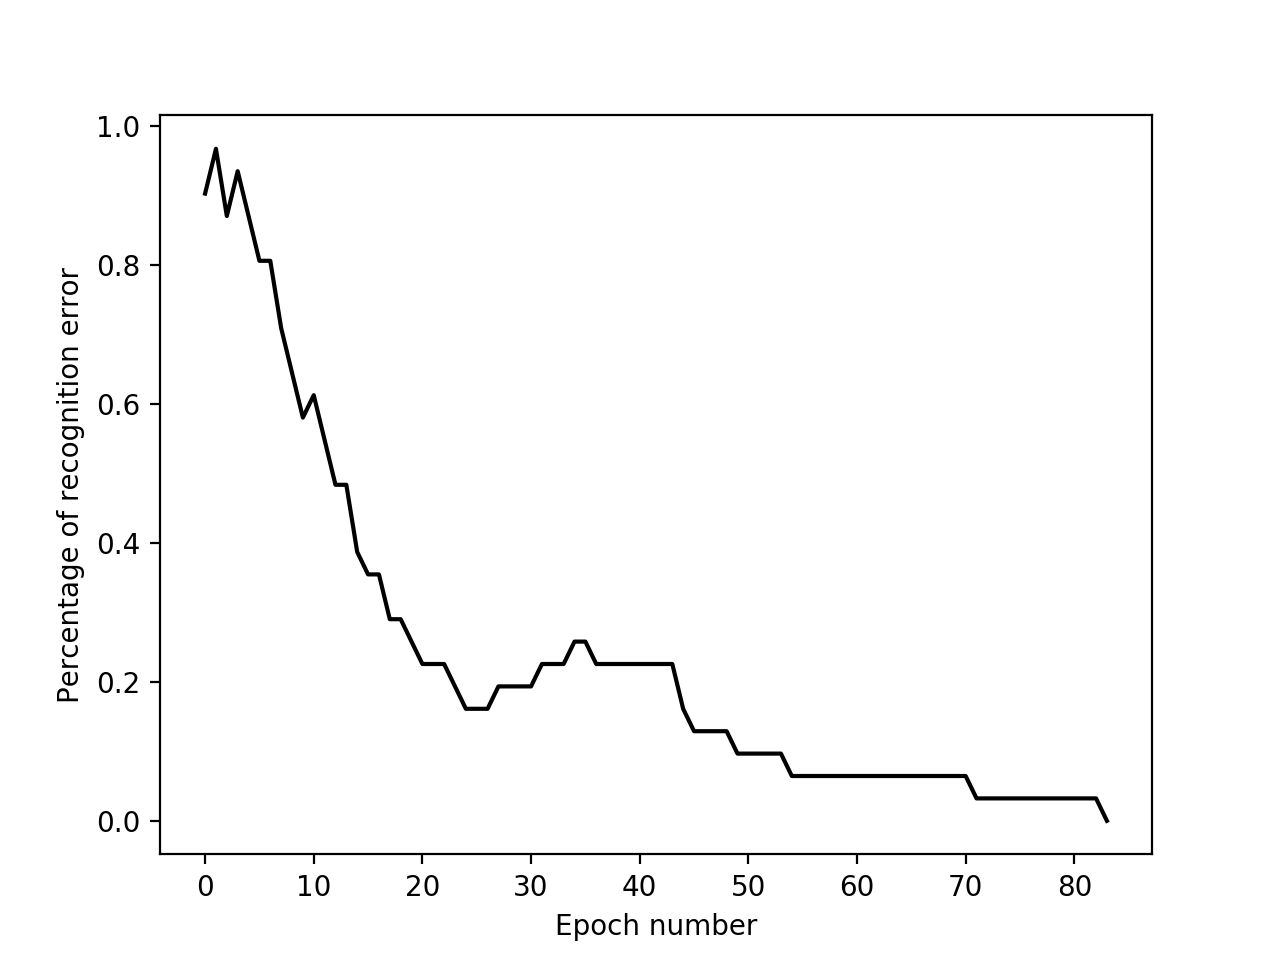
\includegraphics[width=0.9\textwidth]{q2-b-1} % first figure itself
        \caption{Training on perfect data}
    \end{minipage}\hfill
    \begin{minipage}{0.45\textwidth}
    	\centering
         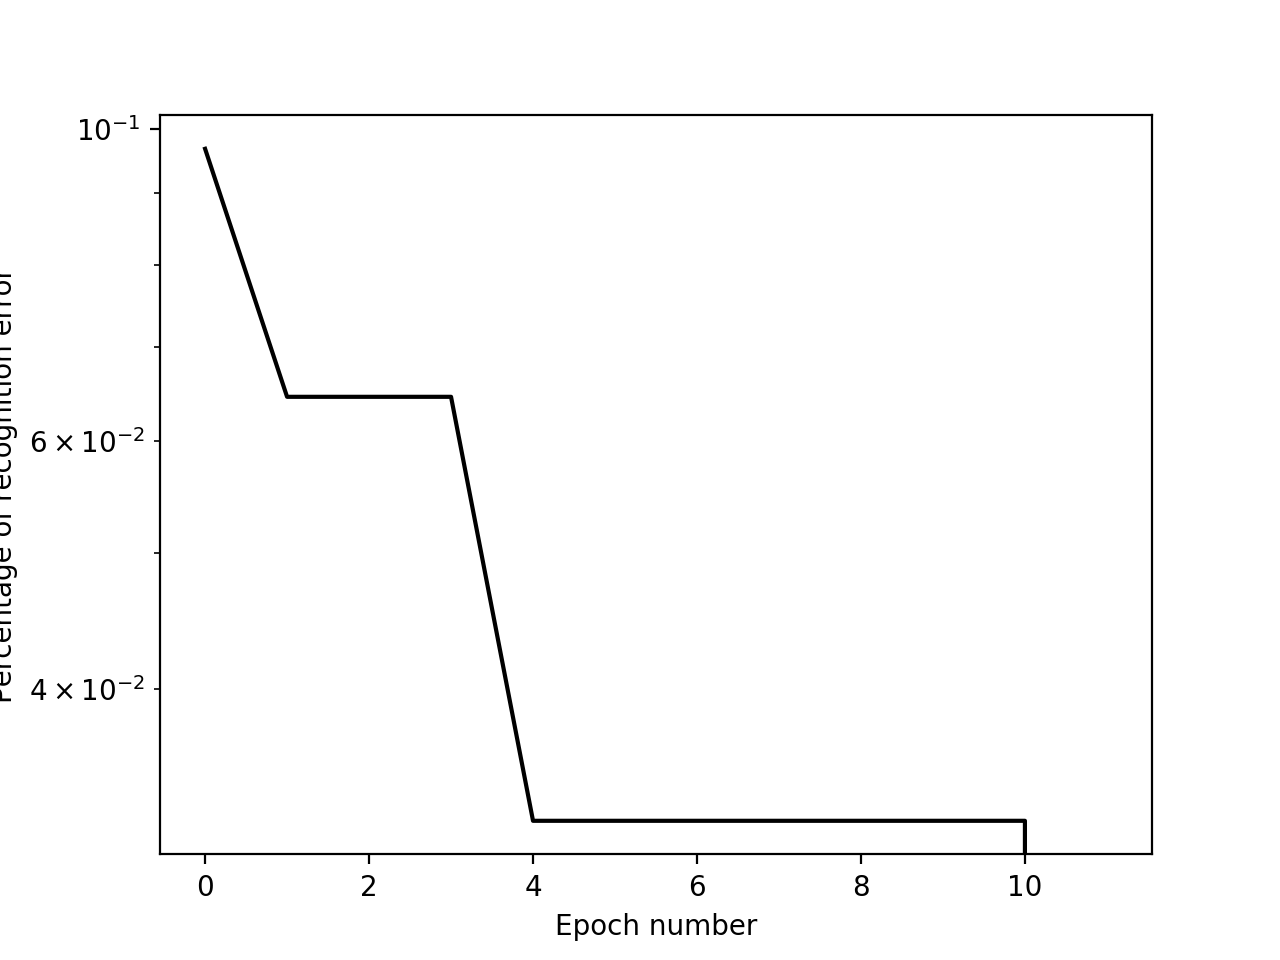
\includegraphics[width=0.9\textwidth]{q2-b-2} % first figure itself
         \caption{Re-training after noisy data}
    \end{minipage}\hfill
\end{figure}

\item The network trained with both perfect and noisy data performed just as well on perfect data, and better on noisy data. The chart below is for the network with 15 neurons.\\
\begin{figure}[h!]
    \centering
     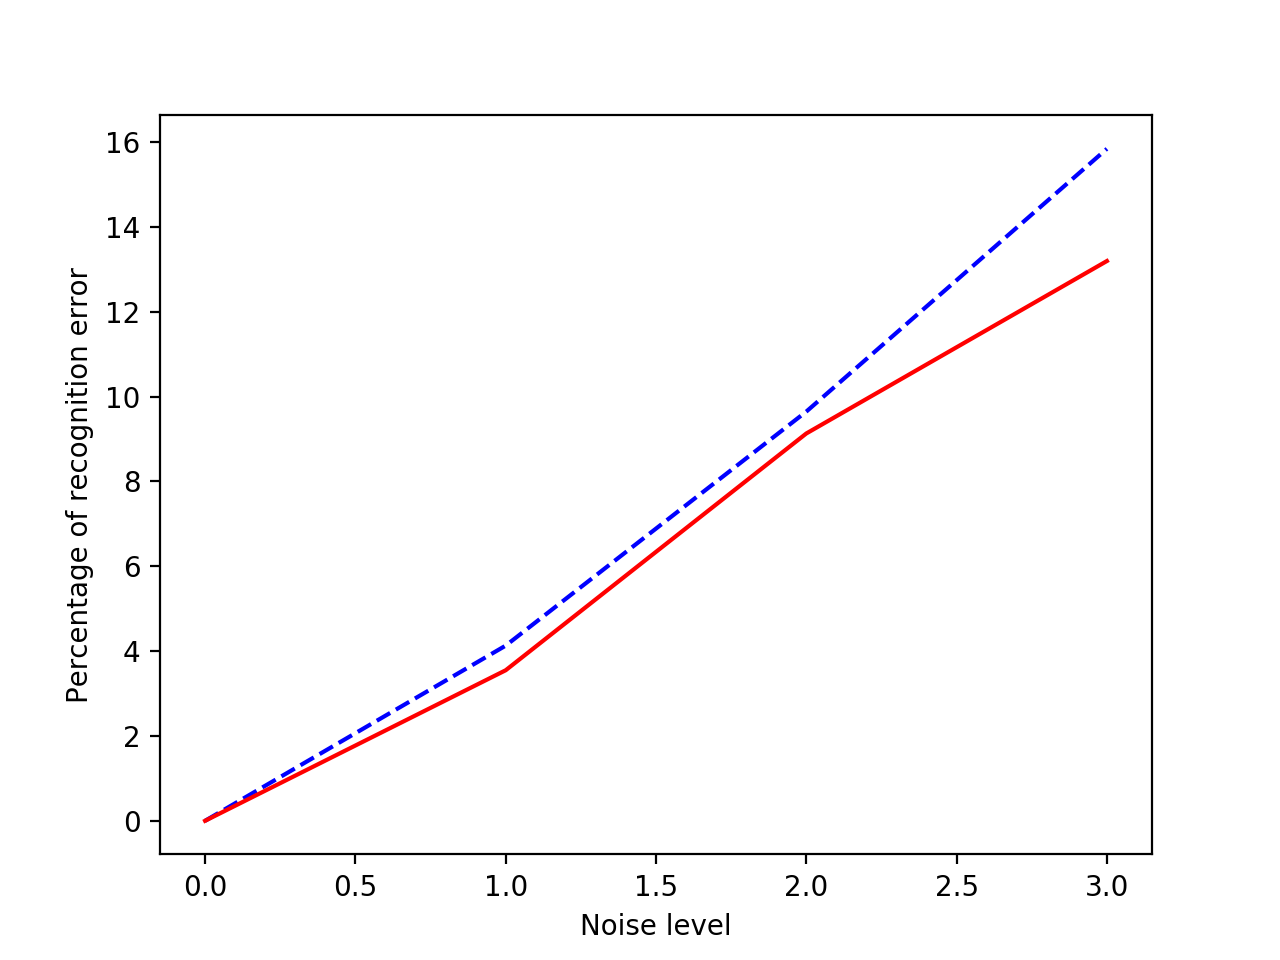
\includegraphics[width=0.5\textwidth]{q2-c}
        \caption{Percentage of Recognition Errors}
\end{figure}

\end{enumerate}

\end{enumerate}
\end{document}